% This is a Basic Assignment Paper but with like Code and stuff allowed in it. 

\documentclass[11pt]{article}
% Preamble

\usepackage[margin=1in]{geometry}
\usepackage{amsfonts, amsmath, amssymb}
\usepackage{fancyhdr, float, graphicx}
\usepackage[utf8]{inputenc} % Required for inputting international characters
\usepackage[T1]{fontenc} % Output font encoding for international characters
\usepackage{fouriernc} % Use the New Century Schoolbook font
\usepackage[nottoc, notlot, notlof]{tocbibind}
\usepackage{listings}
\usepackage{xcolor}

\definecolor{codegreen}{rgb}{0,0.6,0}
\definecolor{codegray}{rgb}{0.5,0.5,0.5}
\definecolor{codepurple}{rgb}{0.58,0,0.82}
\definecolor{backcolour}{rgb}{0.95,0.95,0.92}

\lstdefinestyle{mystyle}{
    backgroundcolor=\color{backcolour},   
    commentstyle=\color{codegreen},
    keywordstyle=\color{magenta},
    numberstyle=\tiny\color{codegray},
    stringstyle=\color{codepurple},
    basicstyle=\ttfamily\footnotesize,
    breakatwhitespace=false,         
    breaklines=true,                 
    captionpos=b,                    
    keepspaces=true,                 
    numbers=left,                    
    numbersep=5pt,                  
    showspaces=false,                
    showstringspaces=false,
    showtabs=false,                  
    tabsize=2
}

\lstset{style=mystyle}

% Header and Footer
\pagestyle{fancy}
\fancyhead{}
\fancyfoot{}
\fancyhead[L]{\textit{\Large{OOPJC Assignment 7}}}
%\fancyhead[R]{\textit{something}}
\fancyfoot[C]{\thepage}
\renewcommand{\footrulewidth}{1pt}



% Other Doc Editing
% \parindent 0ex
%\renewcommand{\baselinestretch}{1.5}

\begin{document}

\begin{titlepage}
	\centering

	%---------------------------NAMES-------------------------------

	\huge\textsc{
		MIT World Peace University
	}\\

	\vspace{0.75\baselineskip} % space after Uni Name

	\LARGE{
		Object Oriented Programming with Java and C++\\
		Second Year B. Tech, Semester 1
	}

	\vfill % space after Sub Name

	%--------------------------TITLE-------------------------------

	\rule{\textwidth}{1.6pt}\vspace*{-\baselineskip}\vspace*{2pt}
	\rule{\textwidth}{0.6pt}
	\vspace{0.75\baselineskip} % Whitespace above the title



	\huge{\textsc{
			Applet Using Java and HTML
		}} \\



	\vspace{0.5\baselineskip} % Whitespace below the title
	\rule{\textwidth}{0.6pt}\vspace*{-\baselineskip}\vspace*{2.8pt}
	\rule{\textwidth}{1.6pt}

	\vspace{1\baselineskip} % Whitespace after the title block

	%--------------------------SUBTITLE --------------------------	

	\LARGE\textsc{
		Practical Report\\
		Assignment 9
	} % Subtitle or further description
	\vfill

	%--------------------------AUTHOR-------------------------------

	Prepared By
	\vspace{0.5\baselineskip} % Whitespace before the editors

	\Large{
		Krishnaraj Thadesar \\
		Cyber Security and Forensics\\
		Batch A1, PA 20
	}


	\vspace{0.5\baselineskip} % Whitespace below the editor list
	\today

\end{titlepage}


\tableofcontents
\thispagestyle{empty}
\clearpage


\setcounter{page}{1}

\section{Aim and Objectives}
\subsection*{Aim}
Develop an applet that displays a simple message in centre of the screen
\subsection*{Objectives}
\begin{enumerate}
	\item To understand concept of Java Applets
	\item To explore features of applets to develop web applications
\end{enumerate}
// Krishnaraj Thadesar
// Batch A1, PA20
// OOPCJ Assignment 9
\section{Problem Statements}
Write a Java applet program that displays a simple message in centre of the screen.

\section{Theory}
%  Introduction to an Applet and its features
% 
%  The Lifecycle of an Applet
% 
%  Discuss about applet tag and its importance
% 
%  Explain various methods of Applet class with necessary examples.

\section{Platform}
\textbf{Operating System}: Arch Linux x86-64 \\
\textbf{IDEs or Text Editors Used}: Visual Studio Code\\
\textbf{Compilers} : g++ and gcc on linux for C++, and javac, with JDK 18.0.2 for Java\\

\section{Output}
The Applet with some text written on it being displayed on the screen.
\begin{figure}[H]
	\centering
	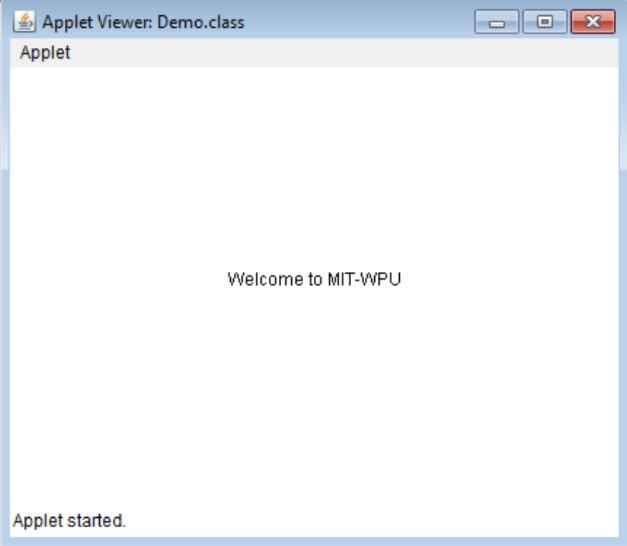
\includegraphics[scale=0.7]{applet.png}
	\caption{}
\end{figure}

\section{Code}

\lstinputlisting[language=java, caption=applet.java]{../Programs/java_implementations/assignment_9/assignment_9.java}
\lstinputlisting[language=html, caption=applet.html]{../Programs/java_implementations/assignment_9/assignment_9.html}

\section{Conclusion}
Thus, developed an applet that displays a simple message in centre of the screen.

\pagebreak

\section{FAQs}
\begin{enumerate}
	\item \textit{What are the restrictions imposed on Java applets?}

	\item \textit{What is the applet class loader, and what does it provide?}

	\item \textit{What is the applet security manager, and what does it provide?}

	\item \textit{Explain the following with suitable examples}

	      \begin{enumerate}
		      \item \textbf{Creating an applet}
		      \item \textbf{Passing parameters to applets}
		      \item \textbf{Adding graphics and colors to applets.}
	      \end{enumerate}
\end{enumerate}
\end{document}